% References:
%
% - About preventing and requesting page breaks:
%   <http://www.tex.ac.uk/cgi-bin/texfaq2html?label=nopagebrk>
%
% - About setting whitespace around display math
%   <http://www.latex-community.org/forum/viewtopic.php?f=47&t=15371#p56484>
%
% - About macros containing paragraphs
%   <http://tex.stackexchange.com/questions/1050/whats-the-difference-between-newcommand-and-newcommand>
%
% - Drawing circles around things
%   http://tex.stackexchange.com/questions/7032/good-way-to-make-textcircled-numbers
%
% - The Listings Package
%   http://ctan.org/pkg/listings


% -----------------------------------------------------------------------------
% information
% -----------------------------------------------------------------------------

\def \docAuthor {Ben Blazak}
\def \docClass  {CPSC 120}
\def \docSchool {California State University Fullerton}
\def \docTerm   {Spring 2014}
\def \docTitle  {Project 4}


% -----------------------------------------------------------------------------
% document setup
% -----------------------------------------------------------------------------

\documentclass[12pt,letterpaper]{article}

\usepackage[includehead,
            includefoot,
            margin=1in,
            top=.25in,
            headheight=.75in,
            headsep=.25in,
            footskip=.25in,
           ]{geometry}

\usepackage[fleqn]{amsmath}
\usepackage{amssymb}
\usepackage{courier}
\usepackage{enumitem}
\usepackage{fancybox}
\usepackage{fancyhdr}
\usepackage{graphicx}
\usepackage{hyperref}
\usepackage{l3regex}
\usepackage{mathtools}
\usepackage{multicol}
\usepackage[normalem]{ulem}
\usepackage[x11names]{xcolor}

\usepackage{tikz}

\usepackage{listings}


% text ------------------------------------------------------------------------

\binoppenalty = 10000  % never break next to a binary operator
\relpenalty   = 10000  % never break next to a relation operator

\setlength{\parindent}{0em}
\setlength{\parskip}{1ex}

\setlist[itemize]{nosep,itemsep=.5ex,parsep=.5ex}

% math ------------------------------------------------------------------------

\setlength{\mathindent}{1cm}

% - "\begin{document}" resets these values, so they have to be treated
%   specially
\AtBeginDocument{
  \setlength{\abovedisplayskip}{1.5ex plus .5ex minus .5ex}
  \setlength{\belowdisplayskip}{1.5ex plus .5ex minus .5ex}
}

% source code -----------------------------------------------------------------

\lstset{
  basicstyle=\ttfamily,
  keywordstyle=\color{Firebrick3},
  commentstyle=\color{blue},
}

% header and footer -----------------------------------------------------------

\pagestyle{fancy}

\lhead{\docClass}
\rhead{\docTitle}
\cfoot{\thepage}
\renewcommand{\headrule}{\hrule height 0.4pt}
\renewcommand{\footrule}{\hrule height 0.4pt}

\fancypagestyle{firstpage}{
  \fancyhead[L]{\docAuthor\\\docClass}
  \fancyhead[C]{\docSchool\\}
  \fancyhead[R]{\docTerm\\\docTitle}
}


% -----------------------------------------------------------------------------
% macros
% -----------------------------------------------------------------------------

% abbreviations ---------------------------------------------------------------

\def \<{\langle}
\def \>{\rangle}

\def \ε{\varepisilon}
\def \θ{\vartheta}
\def \κ{\varkappa}
\def \π{\varpi}
\def \ρ{\varrho}
\def \σ{\varsigma}
\def \φ{\varphi}

\def \Γ{\varGamma}
\def \Δ{\varDelta}
\def \Θ{\varTheta}
\def \Λ{\varLambda}
\def \Ξ{\varXi}
\def \Π{\varPi}
\def \Σ{\varSigma}
\def \Υ{\varUpsilon}
\def \Φ{\varPhi}
\def \Ψ{\varPsi}
\def \Ω{\varOmega}

% special characters ----------------------------------------------------------

\catcode `α = \active \let α \alpha
\catcode `β = \active \let β \beta
\catcode `γ = \active \let γ \gamma
\catcode `δ = \active \let δ \delta
\catcode `ε = \active \let ε \epsilon
\catcode `ζ = \active \let ζ \zeta
\catcode `η = \active \let η \eta
\catcode `θ = \active \let θ \theta
\catcode `ι = \active \let ι \iota
\catcode `κ = \active \let κ \kappa
\catcode `λ = \active \let λ \lambda
\catcode `μ = \active \let μ \mu
\catcode `ν = \active \let ν \nu
\catcode `ξ = \active \let ξ \xi
\catcode `ο = \active \let ο o
\catcode `π = \active \let π \pi
\catcode `ρ = \active \let ρ \rho
\catcode `σ = \active \let σ \sigma
\catcode `τ = \active \let τ \tau
\catcode `υ = \active \let υ \upsilon
\catcode `φ = \active \let φ \phi
\catcode `χ = \active \let χ \chi
\catcode `ψ = \active \let ψ \psi
\catcode `ω = \active \let ω \omega

\catcode `Α = \active \let Α A
\catcode `Β = \active \let Β B
\catcode `Γ = \active \let Γ \Gamma
\catcode `Δ = \active \let Δ \Delta
\catcode `Ε = \active \let Ε E
\catcode `Ζ = \active \let Ζ Z
\catcode `Η = \active \let Η H
\catcode `Θ = \active \let Θ \Theta
\catcode `Ι = \active \let Ι I
\catcode `Κ = \active \let Κ K
\catcode `Λ = \active \let Λ \Lambda
\catcode `Μ = \active \let Μ M
\catcode `Ν = \active \let Ν N
\catcode `Ξ = \active \let Ξ \Xi
\catcode `Ο = \active \let Ο O
\catcode `Π = \active \let Π \Pi
\catcode `Ρ = \active \let Ρ P
\catcode `Σ = \active \let Σ \Sigma
\catcode `Τ = \active \let Τ T
\catcode `Υ = \active \let Υ \Upsilon
\catcode `Φ = \active \let Φ \Phi
\catcode `Χ = \active \let Χ X
\catcode `Ψ = \active \let Ψ \Psi
\catcode `Ω = \active \let Ω \Omega

% other -----------------------------------------------------------------------

% - sometimes a "\par", especially at the end of a block, is necessary to
%   prevent an extra (empty) paragraph from appearing in the output
% - `\color{.!50}` means 50 percent of the current color

     \def \note     #1{{\color{.!50}#1\par}}
\long\def \longnote #1{{\color{.!50}#1\par}}

\long\def \answer #1{
  \filbreak\par #1 \par
}


% -----------------------------------------------------------------------------
% document
% -----------------------------------------------------------------------------

\begin{document}
\thispagestyle{firstpage}


\section*{Numbers to Words}

This project will deal with conditionals, loops, and random numbers.


\filbreak
\subsection*{Turn in}

\begin{itemize}
  \item On Titanium: Your solution as a single PDF composed of
    \begin{itemize}
      \item Your .cpp file
      \item Screenshots of 5 runs of your program
    \end{itemize}
  \item In class: The same document, printed
\end{itemize}


\filbreak
\subsection*{Rules}

\begin{itemize}
  \item If your solution uses arrays then it must not use loops (i.e., it must
    be fully recursive).
  \item Functions are optional, but recommended.
  \item Please try to design the algorithm on your own, or with other students,
    or with help from us.
  \item You may, randomly, be required to explain and justify your algorithm,
    and any code you write.  If you're worried you might forget something,
    please comment your code so that you don't.
\end{itemize}


\filbreak
\subsection*{Suggestions}

\begin{itemize}
  \item Look up the \lstinline{rand()} and \lstinline{srand()} functions.
  \item Recall the modulus operator (\lstinline{%}), integer division, and
      switch statements.
  \item Think carefully about which type of loop would most cleanly do what you
    want.  If you're not sure, and you have time, try all three.
  \item Don't be afraid to use the member functions of \lstinline{std::string},
    if you need them:
    \url{http://en.cppreference.com/w/cpp/string/basic_string}.
  \item Be sure to include the header files declaring the functions that you're
    trying to use!
\end{itemize}


\filbreak
\subsection*{Requirements}

In comments at the top of your code, please include:
\begin{itemize}
  \item Your name.
  \item The assignment (i.e., ``\docTitle'').
  \item Your development environment (including version number).
  \item A list of any nontrivial references you consulted while writing your
    solution.
  \item A list of any notes you have regarding the assignment or your solution.
    \begin{itemize}
      \item This should include a short discussion of any issues you ran into
        while using \lstinline{rand()}, or testing your program.  Are there any
        limitations of \lstinline{rand()} that you happened to notice?
    \end{itemize}
  \item A pseudocode description of your algorithm, written as if to explain
    your ideas to an average classmate without previous knowledge of the
    assignment.
\end{itemize}

Your code must:
\begin{itemize}
  \item Use standard C++ functions to obtain two pseudo-random integers that
    are \textit{not} the same on every run of the program.
    \begin{itemize}
      \item The first should be called \lstinline{start}, and should be between
        $-2^{31}$ and $2^{31}-1$, inclusive.
      \item The second should be called \lstinline{offset}, and should be
        between 2 and 8, inclusive.
    \end{itemize}
  \item Print out a message indicating the value of \lstinline{start}.
  \item Print out a message indicating the value of \lstinline{offset}.
  \item Print out (each on its own line) the English form of the integer
    \lstinline{start}, and every third integer after that until
    \lstinline{offset} integers have been printed.
\end{itemize}


\filbreak
\subsection*{Sample Screenshot}
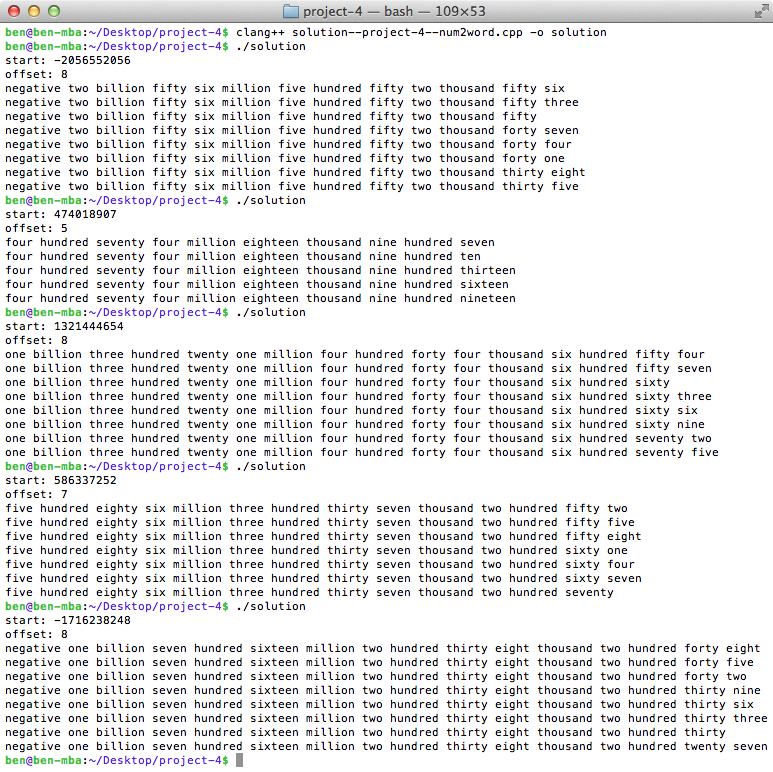
\includegraphics[width=\linewidth]{sample-output.png}


\end{document}

